\subsection{Optimización con y sin gradientes}

La optimización paramétrica sin el uso de gradientes no es escalable para
problemas con un gran número de variables de diseño, como ocurre por ejemplo en
control óptimo, optimización topológica, o aprendizaje automático.

Los algoritmos libres de gradiente avanzan hacia el óptimo poblando el espacio
de diseño y evaluando la función objetivo en estos puntos, para construir una
representación o estadística del entorno que les permita recorrerlo en una
secuencia de pasos. Sin embargo, al introducir más variables de diseño, el
espacio crece exponencialmente, y por tanto el número de puntos a evaluar. Este
fenómeno se conoce como 'la maldición de la dimensionalidad'.

El volumen de un hipercubo n-dimensional, que podemos pretender representa
nuestro espacio de diseño, se expresa como:

\begin{equation}
	V = l^n
\end{equation}

donde $l$ es la longitud del lado y $n$ es la dimensión.


\begin{figure}[h] \centering
	\centering
	\includesvg[width=0.6\textwidth]{./capitulos/metodologia/images/volume_curse_of_dimensionality_print}
	\caption{Crecimiento exponencial del número de puntos a poblar con el número de dimensiones.}
	\label{fig:hypercube}
\end{figure}

Asumiendo que la evaluación de cada punto tiene un coste computacional no
despreciable, el uso de estos algoritmos se vuelve inviable para problemas con
más de unas pocas decenas de variables de diseño (figura
\ref{fig:gradient_based_vs_gradient_free}). Por el contrario, los algoritmos
basados en gradientes no requieren poblar el espacio de diseño para encontrar
una dirección hacia el óptimo. Emplean los gradientes de la funcion objetivo
respecto de las variables de diseño como guía, y su obtención es independiente
del número de incógnitas, como veremos con la diferenciación automática y
derivadas adjuntas.

Esta estrategia permite la optimización de problemas con un elevado número de
incógnitas. Por ejemplo, el modelo de lenguaje Llama-3.1-405b de Meta utiliza
405 mil millones de variables \cite{dubey2024llama}, o parámetros como se
conocen en el contexto del aprendizaje automático.

\begin{figure}[h]
	\centering
	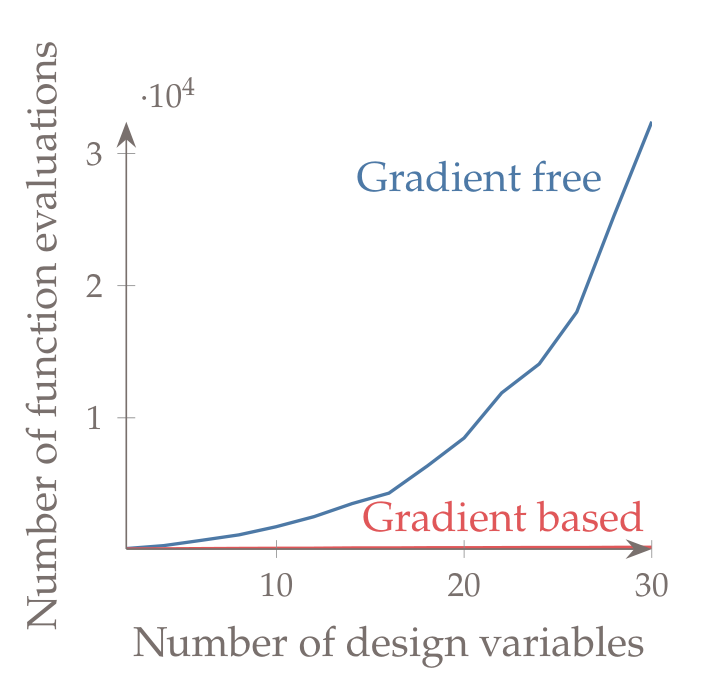
\includegraphics[width=0.4\textwidth]{./capitulos/metodologia/images/gradient_based_vs_gradient_free.png}
	\caption{Los algoritmos de optimización que emplean gradientes escalan mucho mejor con el número de variables de diseño (Adaptado de Martins y Ning \cite{mdobook}, p. 22).}
	\label{fig:gradient_based_vs_gradient_free}
\end{figure}

Por otro lado, y sin importar la técnica escogida para orientarse en el entorno
de diseño, la trayectoria desde el punto inicial al final crece con la
dimensión, pero no de forma tan drástica. La diagonal de un hipercubo
n-dimensional viene dada por:

\begin{equation}
	d = l\sqrt{n}
\end{equation}

Nótese que el aumento no es exponencial con el número de dimensiones, ni tan
siquiera lineal.

Si el número de iteraciones realizadas por el algoritmo de optimización es
proporcional a la longitud del camino entre los puntos inicial y final(óptimo),
entonces el coste computacional se incrementa con la raiz del número de
dimensiones, o variables de diseño.

\subsection{Problemas con restricciones y condiciones de primer orden}

La gran mayoría de los problemas en ingeniería requieren el uso de
restricciones en su formulación. Estas restricciones pueden ser de igualdad o
desigualdad y representan limitaciones físicas, económicas o de diseño que
deben satisfacerse durante el proceso de optimización.

Mientras que en la resolución de problemas sin restricciones frecuentemente se
usan métodos quasi-Newton como BFGS, u otros populares en el ámbito del
deep-learning como Adam \cite{kingma2014adam}, aquí el planteamiento es algo
diferente, empezando por las condiciones de primer orden para el óptimo.

Considerando inicialmente solo restricciones de igualdad, en el óptimo
restringido se tendrá:

\begin{equation}
	f(x^* + p) \approx f(x^*) + \nabla f(x^*)^T p
\end{equation}

Si $x^*$ es un punto mínimo, entonces cada punto en un pequeño entorno debe
tener un valor mayor:

\begin{equation}
	f(x^* + p) \geq f(x^*)
\end{equation}

Por lo tanto:

\begin{equation}
	\nabla f(x^*)^T p \geq 0
\end{equation}

Sin embargo, para restricciones de igualdad, si una dirección $p$ es factible,
entonces $-p$ también debe ser factible (figura \ref{fig:constraint_direction}).

\begin{figure}[h] \centering
	\centering
	\includesvg[width=0.6\textwidth]{./capitulos/metodologia/images/constraint_direction}
	\caption{Direcciones válidas a lo largo de la restricción $h$.}
	\label{fig:constraint_direction}
\end{figure}

Esto significa que el gradiente de la función es perpendicular al camino
viable:

\begin{equation} \label{eq:objective_gradient_perpendicular_to_direction_p}
	\nabla f(x^*)^T p = 0
\end{equation}

Ahora, para las restricciones de igualdad:

\begin{equation}
	h_j(x + p) \approx h_j(x) + \nabla h_j(x)^T p
\end{equation}

Y asumiendo que $x$ es un punto que satisface las condiciones de igualdad,
entonces:

\begin{equation}
	h_j(x + p) = h_j(x) = 0
\end{equation}

\begin{equation}
	\nabla h_j(x)^T p = J_h(x) p = 0
\end{equation}

donde $J_h$ es el jacobiano.

Esto significa que $p$ es ortogonal a todos los gradientes de las
restricciones de igualdad. Los gradientes forman un plano, y la dirección
viable es perpendicular a él (figura \ref{fig:constraints_jacobian}).

\begin{figure}[h]
	\centering
	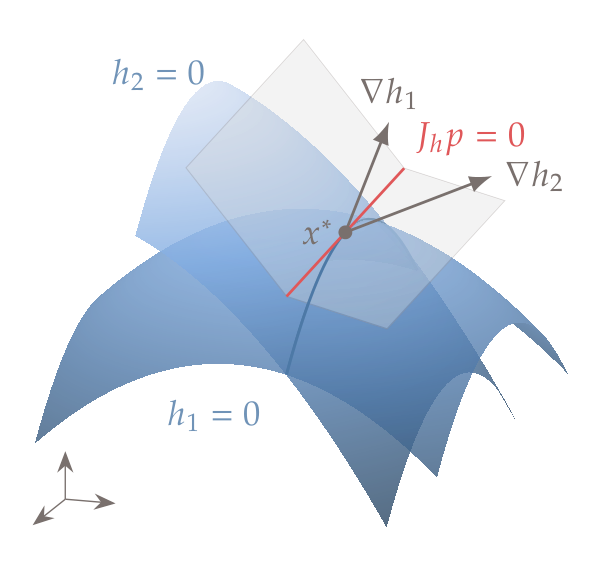
\includegraphics[width=0.4\textwidth]{./capitulos/metodologia/images/constraints_jacobian.png}
	\caption{Los gradientes de las restricciones son perpendiculares a la dirección válida $p$ (Adaptado de Martins y Ning \cite{mdobook}, p. 160).}
	\label{fig:constraints_jacobian}
\end{figure}

Pero en \eqref{eq:objective_gradient_perpendicular_to_direction_p} dijimos que:

\begin{equation}
	\nabla f(x^*)^T p = 0
\end{equation}

Lo que significa que $\nabla f(x^*)^T$ también es ortogonal al camino
factible, y por lo tanto, también está contenido en ese plano formado por los
gradientes de las restricciones de igualdad (figura \ref{fig:gradients_on_the_same_plane}).

\begin{figure}[h]
	\centering
	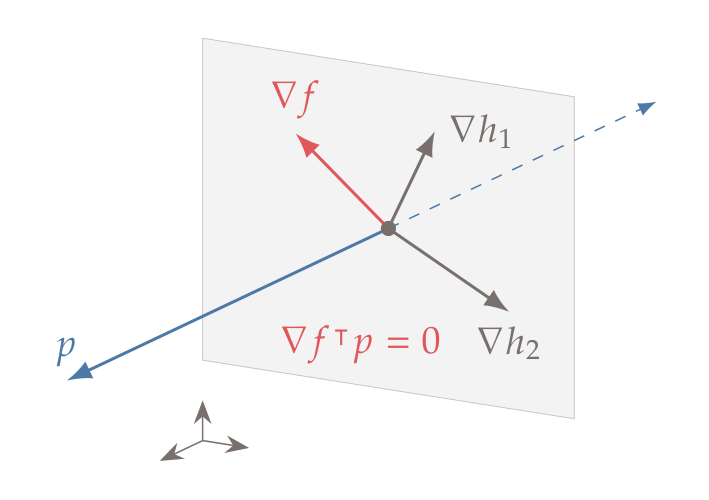
\includegraphics[width=0.4\textwidth]{./capitulos/metodologia/images/gradients_on_the_same_plane.png}
	\caption{Los gradientes de la función objetivo e igualdades son normales a la
		dirección $p$ y están en el mismo plano (Adaptado de Martins y Ning
		\cite{mdobook}, p. 160).}
	\label{fig:gradients_on_the_same_plane}
\end{figure}

Así, $\nabla f(x^*)^T$ puede expresarse como una combinación lineal de los
gradientes de igualdad que forman ese plano.

\begin{equation}
	\nabla f(x^*) = - \sum_{j=1}^{n_h} \lambda_j \nabla h_j(x^*) = - J_h(x)^T \lambda
\end{equation}

donde $\lambda_j$ es el multiplicador de Lagrange para la restricción $j$. Y
las condiciones de optimalidad de primer orden quedan como:

\begin{equation}
	\begin{aligned}
		\nabla f(x^*) & = -J_h(x^*)^T \lambda \\
		h(x)          & = 0
	\end{aligned}
\end{equation}

Pero definiendo hábilmente la función Lagrangiana, obtenemos las mismas
condiciones derivándola respecto de las variables de diseño y los
multiplicadores de Lagrange.

\begin{equation}
	\mathcal{L}(x, \lambda) = f(x) + h(x)^T \lambda
\end{equation}

\begin{equation}
	\begin{aligned}
		\nabla_x \mathcal{L}         & = \nabla f(x) + J_{h(x)}^T \lambda = 0 \\
		\nabla_{\lambda} \mathcal{L} & = h(x) = 0
	\end{aligned}
\end{equation}

El teorema de Lagrange establece que para cada mínimo restringido de $f$ hay
un punto crítico para $\mathcal{L}$. Pero estos puntos críticos para el
Lagrangiano son puntos de silla, lo que nos impide directamente minimizar la
Lagrangiana con métodos de optimización sin restricciones.

A pesar de la utilidad de la Lagrangiana, no es cierto que nos permita eliminar las
restricciones del problema:

\begin{equation}
	\begin{aligned}
		 & \min
		 &                 & f(x)                         \\
		 & \text{sujeto a}
		 &                 & h_k(x) = 0, \quad \forall k,
	\end{aligned}
	\quad \neq \quad
	\begin{aligned}
		 & \min
		 &      & f(x) + \sum_{k} \lambda_k h_k(x)
	\end{aligned}
\end{equation}

Puede verse intuitivamente porque llevando el valor de los multiplicadores de
Lagrange hacia menos infinito daría un mínimo de menos infinito.

Para considerar restricciones de desigualdad, las podemos convertir en
igualdades añadiendo una variable de holgura no negativa. La desigualdad:

\begin{equation}
	g(x) \leq 0
\end{equation}

equivale a

\begin{equation}
	g(x) + s^2 = 0
\end{equation}

Y las incorporamos igualmente en la función Lagrangiana:

\begin{equation}
	\mathcal{L}(x, \lambda, \sigma, s) = f(x) + \lambda^T h(x) + \sigma^T (g(x) + s \odot s)
\end{equation}

Siendo $\odot$ la multiplicación elemento a elemento.


Pero los multiplicadores de Lagrange de desigualdad $\sigma$ tienen la
peculiaridad de que deben ser no negativos. Esta condición de no negatividad se
aplica como una cota en las condiciones KKT (Karush-Kuhn-Tucker, condiciones
generales de primer orden), que resultan de igualar a cero las derivadas de la
Lagrangiana respecto de sus variables de diseño ($x$, $\lambda$, $\sigma$ y
$s$).

\begin{align}
	\frac{\partial \mathcal{L}}{\partial x}       & = \nabla f + J_h^T \lambda + J_g^T \sigma = 0             \\
	\frac{\partial \mathcal{L}}{\partial \lambda} & = h = 0                                                   \\
	\frac{\partial \mathcal{L}}{\partial \sigma}  & = g + s \odot s = 0                                       \\
	\frac{\partial \mathcal{L}}{\partial s}       & = \sigma \odot s = 0   \label{eq:complementary_slackness} \\
	\sigma                                        & \geq 0
\end{align}

\subsection{Solución de ecuaciones KKT}

Las ecuaciones KKT son necesarias para el óptimo, pero no suficientes para una
función objetivo no convexa, porque aún necesitamos las condiciones de segundo
orden para discernir mínimo de máximo o puntos de inflexión.

Pero en principio podríamos tratar de resolver el sistema de ecuaciones no
lineales con Newton-Raphson, y con las raíces del resultado que tengan todos
los multiplicadores de Lagrange $\sigma$ positivos, explorar la concavidad de
la función objetivo y finalmente solo quedarnos con los mínimos.

Notar que la condición de no negatividad para $\sigma$ no entraría dentro del
sistema a resolver, porque es una desigualdad, y solo se aplicaría después para
cribar las raíces encontradas.

Sin embargo, esta no es la vía comúnmente seguida para atacar el problema,
porque la condición de complementariedad de holgura (ecuación
\eqref{eq:complementary_slackness}), introduce una complejidad que lleva a una
convergencia inestable del algoritmo (Newton-Raphson), y dificultad para elegir
puntos iniciales aceptables.

Si nos fijamos en esta condición:

\begin{equation}
	\sigma \odot s = 0
\end{equation}

implica que para cada desigualdad, su multiplicador $\sigma$ debe ser cero, y/o
la holgura $s$ debe ser cero. Si $s$ es cero, quiere decir que la restricción
es activa (de igualdad), y de lo contrario inactiva. Se da una discontinuidad
en el espacio de soluciones difícil de tratar por Newton-Raphson, que podemos
tratar de visualizar en el cuadro
\ref{tab:complementary_slackness_discontinuity}, donde vemos que al pasar de
una desigualdad activa a inactiva, el multiplicador de Lagrange ha de pasar
instantáneamente a valer 0, aunque la holgura evolucione de forma suave.

\begin{table}[ht]
	\centering
	\caption{Discontinuidad en condición de complementariedad.}
	\label{tab:complementary_slackness_discontinuity}
	\begin{tabular}{@{}lll@{}}
		\toprule
		\textbf{Activo} & \textbf{Inactivo} \\
		\midrule
		$\sigma_1 = 13$ & $\sigma_1 = 0$    \\
		$s_1 = 0$       & $s_1 = 0.01$      \\
		\bottomrule
	\end{tabular}
\end{table}

Por este motivo, la estrategia usualmente empleadada es la de no considerar
desigualdades, simplificando considerablemente el sistema de ecuaciones a
resolver por Newton-Raphson.

Métodos SQP (Sequential Quadratic Programming) a cada iteración estiman qué
desigualdades son activas, y las resuelven como unas condiciones de igualdad
más, mientras que las inactivas no se consideran.

Y algoritmos de punto interior convierten todas las desigualdades en
condiciones de igualdad con el uso de variables de holgura y penalizando con un
método de barrera para mantener su valor mayor que 0.


\subsection{Método de punto interior}

Se pasa de un problema como:

\begin{align}
	\min \quad            & f(\mathbf{x})         \\
	\text{sujeto a} \quad & h(\mathbf{x}) = 0     \\
	                      & g(\mathbf{x}) \leq  0
\end{align}

a

\begin{align}
	\min \quad            & f(\mathbf{x}) - \mu_b \sum_{j=1}^{n_g} \ln s_j \\
	\text{sujeto a} \quad & h(\mathbf{x}) = 0                              \\
	                      & g(\mathbf{x}) + \mathbf{s} = 0
\end{align}

donde $\mu_b$ es un factor para penalizar más o menos el término barrera. Este
término distorsiona la función objetivo, por lo que $\mu_b$ se va haciendo
progresivamente más cercano a 0 para aproximarse al verdadero objetivo conforme
avanza la optimización.

La función Lagrangiana de esta formulación es:

\begin{equation}
	\mathcal{L}(x, \lambda, \sigma, s) = f(x) - \mu_b \mathbf{e}^T \ln s + \lambda^T h(x) + (\sigma^T g(x) + s^T \sigma)
\end{equation}

Con sus correspondientes condiciones de primer orden:

\begin{align}
	\frac{\partial \mathcal{L}}{\partial x}       & = 0 = \nabla f(x) + J_h(x)^T \lambda + J_g(x)^T \sigma \\
	\frac{\partial \mathcal{L}}{\partial \lambda} & = 0 = h                                                \\
	\frac{\partial \mathcal{L}}{\partial \sigma}  & = 0 = g + s                                            \\
	\frac{\partial \mathcal{L}}{\partial s}       & = 0 = -\mu_b S^{-1} e + \sigma
\end{align}

donde $e = [1, \ldots, 1]$ es un vector de $n_g$ unos, introducido para
expresar la suma en forma vectorial, y $S$ es una matriz diagonal con las
variables de holgura como elementos.

Multiplicando la última ecuación por $S$ se tiene un sistema más favorable:

\begin{equation}
	\begin{aligned}
		\nabla f(x) + J_h(x)^T \lambda + J_g(x)^T \sigma & = 0 \\
		h                                                & = 0 \\
		g + s                                            & = 0 \\
		-\mu_b e + S \sigma                              & = 0
	\end{aligned}
\end{equation}

Y ahora con estas ecuaciones residuales se aplica el método de Newton-Raphson:

\begin{equation}
	\begin{bmatrix}
		H_L(x) & J_h(x)^T & J_g(x)^T & 0      \\
		J_h(x) & 0        & 0        & 0      \\
		J_g(x) & 0        & 0        & I      \\
		0      & 0        & S        & \sigma
	\end{bmatrix}
	\begin{bmatrix}
		s_x       \\
		s_\lambda \\
		s_\sigma  \\
		s_s
	\end{bmatrix}
	= -
	\begin{bmatrix}
		\nabla_x \mathcal{L}(x, \lambda, \sigma) \\
		h(x)                                     \\
		g(x) + s                                 \\
		S \sigma - \mu_b e
	\end{bmatrix}
\end{equation}

Finalmente, se observa que si multiplicamos la última ecuación por $S^{-1}$
obtenemos un sistema simétrico, que es más fácil de resolver:

\begin{equation}
	\begin{bmatrix}
		H_L(x) & J_h(x)^T & J_g(x)^T & 0            \\
		J_h(x) & 0        & 0        & 0            \\
		J_g(x) & 0        & 0        & I            \\
		0      & 0        & I        & S^{-1}\Sigma
	\end{bmatrix}
	\begin{bmatrix}
		s_x       \\
		s_\lambda \\
		s_\sigma  \\
		s_s
	\end{bmatrix}
	= -
	\begin{bmatrix}
		\nabla_x \mathcal{L}(x, \lambda, \sigma) \\
		h(x)                                     \\
		g(x) + s                                 \\
		\sigma - \mu_b S^{-1}e
	\end{bmatrix}
\end{equation}

sistema lineal que nos da los pasos (steps) para la próxima iteración $s_x$,
$s_\lambda$, $s_\sigma$ y  $s_s$.

\subsection{Intercambiabilidad entre problemas con y sin restricciones}

Como vimos previamente, la Lagrangiana de un problema nos proporciona las
condiciones de primer orden para la optimalidad de un problema, pero no es una
representación sin restricciones de un problema equivalente con restricciones.

Aunque sí es posible transformar un problema con condiciones en uno sin ellas a
través de otros medios.

Uno de ellos es incorporar las restricciones en la función objetivo como
penalizaciones, como en el método de penalización cuadrática exterior, que
transforma un problema del estilo:

\begin{align}
	\min \quad            & f(\mathbf{x})         \\
	\text{sujeto a} \quad & h(\mathbf{x}) = 0     \\
	                      & g(\mathbf{x}) \leq  0
\end{align}

a otro semejante:

\begin{equation}
	\min \hat{f}(\mathbf{x}; \mu) = f(\mathbf{x}) + \frac{\mu_h}{2} \sum_{l=1}^{n_h} h_l(\mathbf{x})^2 + \frac{\mu_g}{2} \sum_{j=1}^{n_g} \max(0, g_j(\mathbf{x}))^2
\end{equation}

con factores $\mu_h$ y $\mu_g$ para los términos que violan las condiciones de
igualdad y desigualdad respectivamente, cuyos valores se aumentan a la vez que
evoluciona la optimización hacia el óptimo para penalizar de forma más estricta
el incumplimiento de las restricciones.

Otro modo sería primero transformar las inigualdades en igualdades, y después
tratar las restricciones como un sistema de ecuaciones a resolver, cuyas
soluciones son valores de los que depende la función objetivo.

De nuevo, partiendo del problema modelo:

\begin{align}
	\min_{\mathbf{x}} \quad & f(\mathbf{x}, \mathbf{y})         \\
	\text{sujeto a} \quad   & h(\mathbf{x}, \mathbf{y}) = 0     \\
	                        & g(\mathbf{x}, \mathbf{y}) \leq  0
\end{align}

de forma similar al método de punto interior, usamos
variables de holgura para solo considerar restricciones
de igualdad:

\begin{align}
	\min_{\mathbf{x}, \mathbf{s}} \quad & f(\mathbf{x}, \mathbf{y}) - \mu_b \sum_{j=1}^{n_g} \ln s_j \\
	\text{sujeto a} \quad               & h(\mathbf{x}, \mathbf{y}) = 0                              \\
	                                    & g(\mathbf{x}, \mathbf{y}) + \mathbf{s} = 0
\end{align}

y aquí observamos que las restricciones pueden representarse como un sistema
de ecuaciones, con las variables de diseño $x$ como entradas, y variables
de estado $y$ como incógnitas. Si tuviéramos una función que nos devolviese
estas:

\begin{equation}
	u = \text{resuelve\_sistema}(x)
\end{equation}

entonces el problema anterior se podría reescribir como:

\begin{align} \label{eq:optimization_with_system_solving}
	\min_{\mathbf{x}, \mathbf{s}} \quad & f(\mathbf{x}, \text{resuelve\_sistema}(x)) - \mu_b \sum_{j=1}^{n_g} \ln s_j
\end{align}

Obteniendo $y$ a través de la función $\text{resuelve\_sistema}$ no necesitamos las restricciones.

Esta transformación también se ilustra en la imagen \ref{fig:constraints_to_no_constraints}.

\begin{figure}[h]
	\centering
	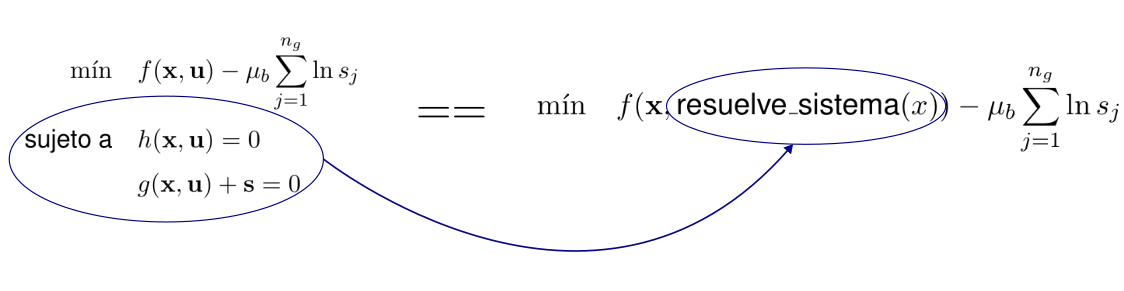
\includegraphics[width=0.9\textwidth]{./capitulos/metodologia/images/constraints_to_no_constraints.png}
	\caption{Transformación de problema con restricciones a no restricciones.}
	\label{fig:constraints_to_no_constraints}
\end{figure}

\subsection{Ecuaciones en derivadas parciales como restricciones}

Cuando resolvemos ecuaciones en derivadas parciales, normalmente se acude al
uso de un paquete de software para su solución. El usuario proporciona una
geometría, unas condiciones de frontera, condiciones iniciales, selecciona
propiedades para materiales, y otras opciones a través de la interfaz, y a
cambio el programa ensambla un sistema de ecuaciones que puede ser lineal, no
lineal, o un sistema de ecuaciones diferenciales o de ecuaciones diferenciales
y algebraicas en estudios con transitorios.

Por ejemplo, en el caso de un análisis de equilibrio estático, partimos de las
ecuaciones de equilibrio dinámico de la mecánica de sólidos:

\begin{equation}
	\nabla \cdot \sigma + \rho b = \rho \frac{\partial^2 y}{\partial t^2} + c \frac{\partial y}{\partial t}
\end{equation}

donde $\sigma$ es el tensor de tensiones, $\rho$ la densidad del material, $b$
el vector de fuerzas másicas (i.e. gravedad), $y$ los desplazamientos, y $c$ el
coeficiente de fricción.

Que para el caso estático se simplifica a:

\begin{align}
	\frac{\partial \sigma_{11}}{\partial x_1} + \frac{\partial \sigma_{12}}{\partial x_2} + \frac{\partial \sigma_{13}}{\partial x_3} + \rho b_1 = 0 \\
	\frac{\partial \sigma_{21}}{\partial x_1} + \frac{\partial \sigma_{22}}{\partial x_2} + \frac{\partial \sigma_{23}}{\partial x_3} + \rho b_2 = 0 \\
	\frac{\partial \sigma_{31}}{\partial x_1} + \frac{\partial \sigma_{32}}{\partial x_2} + \frac{\partial \sigma_{33}}{\partial x_3} + \rho b_3 = 0
\end{align}

Un código numérico de elementos finitos divide el dominio de interés en
elementos, aproxima las soluciones con polinomios base, construye la matriz
elemental para cada elemento con la forma débil de las ecuaciones, y al final
ensambla las matrices y aplica condiciones de frontera, para producir el
sistema de ecuaciones:

\begin{equation} \label{eq:static_analysis_system}
	K y = f
\end{equation}

$K$ es la matriz de rigidez, $f$ las fuerzas aplicadas, y $y$ los
desplazamientos de los nodos buscados.

Empleando un software de elementos finitos, el programa típicamente nos
proporciona los desplazamientos solución, pero no expone las ecuaciones del
sistema formado.

De esta forma, cuando formulamos un problema de optimización restringido por
ecuaciones en derivadas parciales, al no tener acceso al sistema de ecuaciones
empleado, como podría ser \eqref{eq:static_analysis_system}, no podemos
incorporarlas como restricciones, y nuestro problema adquiere la forma de
\eqref{eq:optimization_with_system_solving}.

Para un análisis nos bastaría con que el código nos diera las soluciones $y$,
pero en un problema de optimización necesitamos además los gradientes de la
función $\text{resuelve\_sistema}$ a través del sistema de ecuaciones respecto
de las variables de diseño.
